\Chapter{Számítási idő}
A függvénykönyvtár, illetve a demo program futási idejét 2 különböző módon tesztelhetjük. Első esetben csak a háromszögek metszéspontjának számítása lett figyelembe véve, míg a második esetben az OpenGL \cite{OpenGL} renderelési ideje is.
A számítások intel core i9-13900 processzoron, illetve RTX 4070 videókártyán lettek elvégezve. Az eredmények más rendszereken mások lehetnek. Modellek ütközésének vizsgálatakor mindig 1 kockát (12 háromszög) és több hengert (124 háromszög * modellek száma) vettünk figyelembe.
\begin{figure}[h]
	\centering
	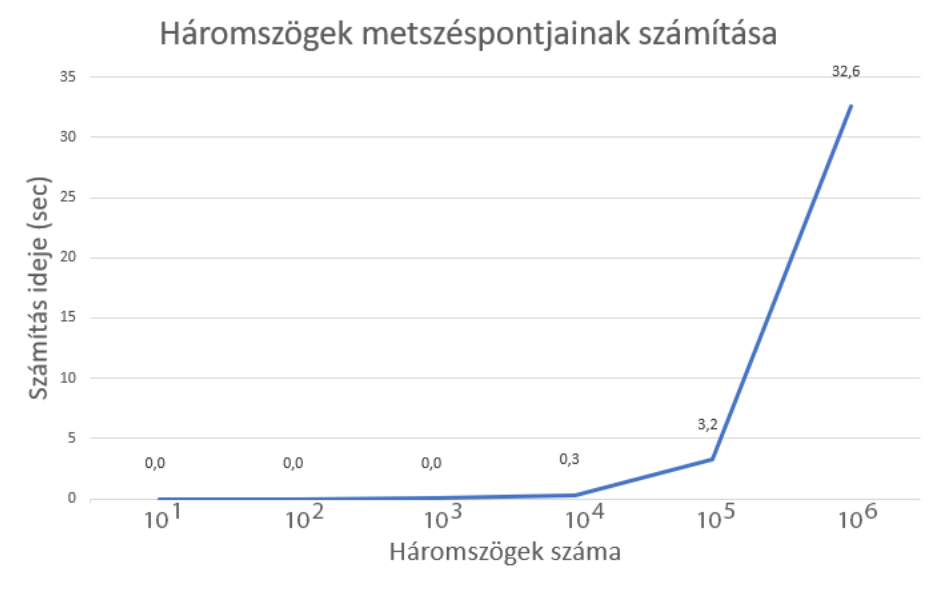
\includegraphics[width=15truecm, height=9truecm]{images/háromszögek_száma.png}
	\caption{Háromszögek metszéspontjának számítása}
	\label{fig:szam_1}
\end{figure}

Háromszögek metszéspontjainak számítási idejét láthatjuk a \ref{fig:szam_1} ábrán, ahogy a számítási idő lineárisan nő a háromszögek száma alapján.

\newpage

\begin{figure}[h]
	\centering
	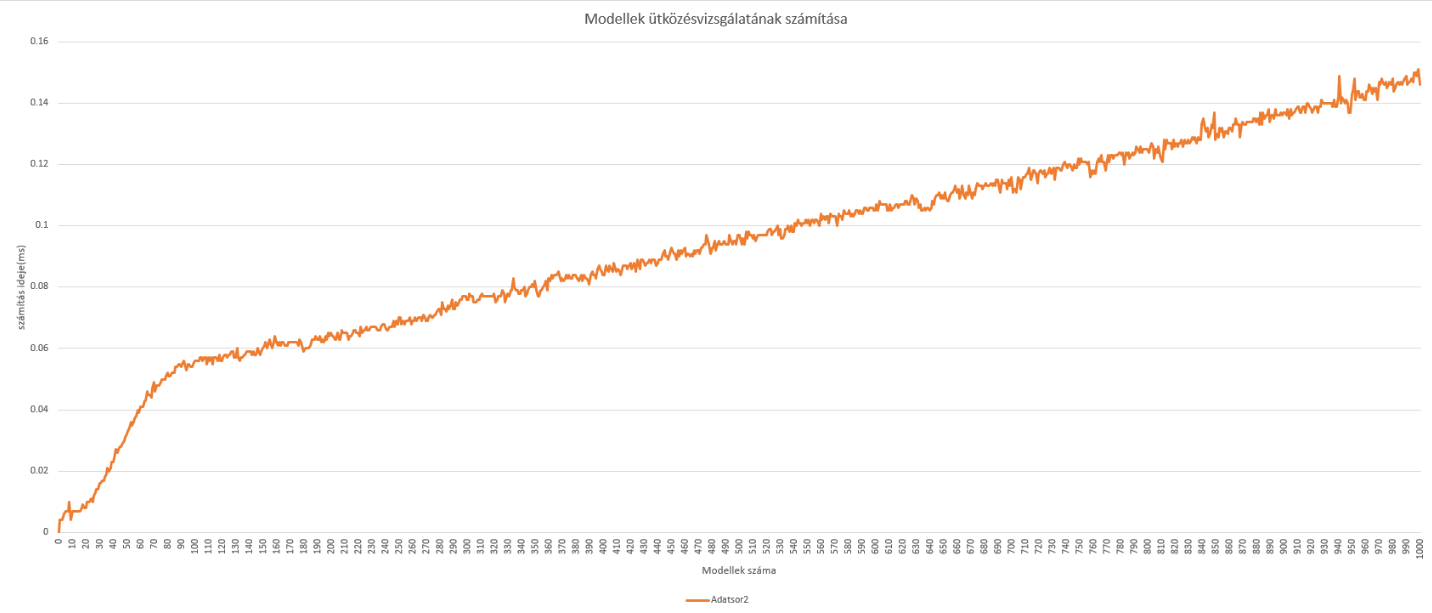
\includegraphics[width=15truecm, height=9truecm]{images/modellek_számítása.png}
	\caption{Modellek ütközésvizsgálatának számítása}
	\label{fig:szam_2}
\end{figure}

Modellek ütközésvizsgálatánál már nem mondhatjuk el, hogy teljesen lineáris lenne a számítási igény. Az elején a \ref{fig:szam_2} ábrán (kb. 100 modellig) hirtelen nő a számítási idő, majd egyre inkább egyenletes lesz, lineárisan nő a szükséges idő.